\section{MOOT-PID, multi-objetive optimization tool for PID controllers}
\label{sec:results}
%
An application that allows the user to optimally tune \gls{2dof} \gls{pid} using a \gls{soptd} model for the plant was developed. Since all the results in the obtained database are optimal from a Pareto standpoint, it is necessary to provide the user with a tool to select the final tuning of the controller.

The user has to provide the following inputs:
\begin{enumerate}
	\item A plant model in the form of a \gls{soptd} transfer function.
	\item A desired robustness (given by the maximum sensitivity).
	\item The allowed degradation of each cost function. The user can choose a degradation level from zero to one for each cost function ($J_r$, $J_{di}$, $J_{do}$). A value of zero means no degradation and one represents a total degradation. One of the cost functions needs to have a degradation of zero. If this is not true, the program automatically finds the lowest value of $J_{di}$.
\end{enumerate}
%
The tool then provides the Pareto-optimal tuning along with a simulation of the closed-loop response. It has to be noticed that the tool interpolates only from the Pareto front. Even if the user let any function to have a degradation of 1, the tuning still is Pareto optimal. Therefore, the performance of the closed loop will be better (in the Pareto sense and with the given constraints) than any other possible parameter combinations.

\subsection{Presentation of the tool}
The main window is shown in %
%
\begin{figure}%[t]%[ht]
	\centering
	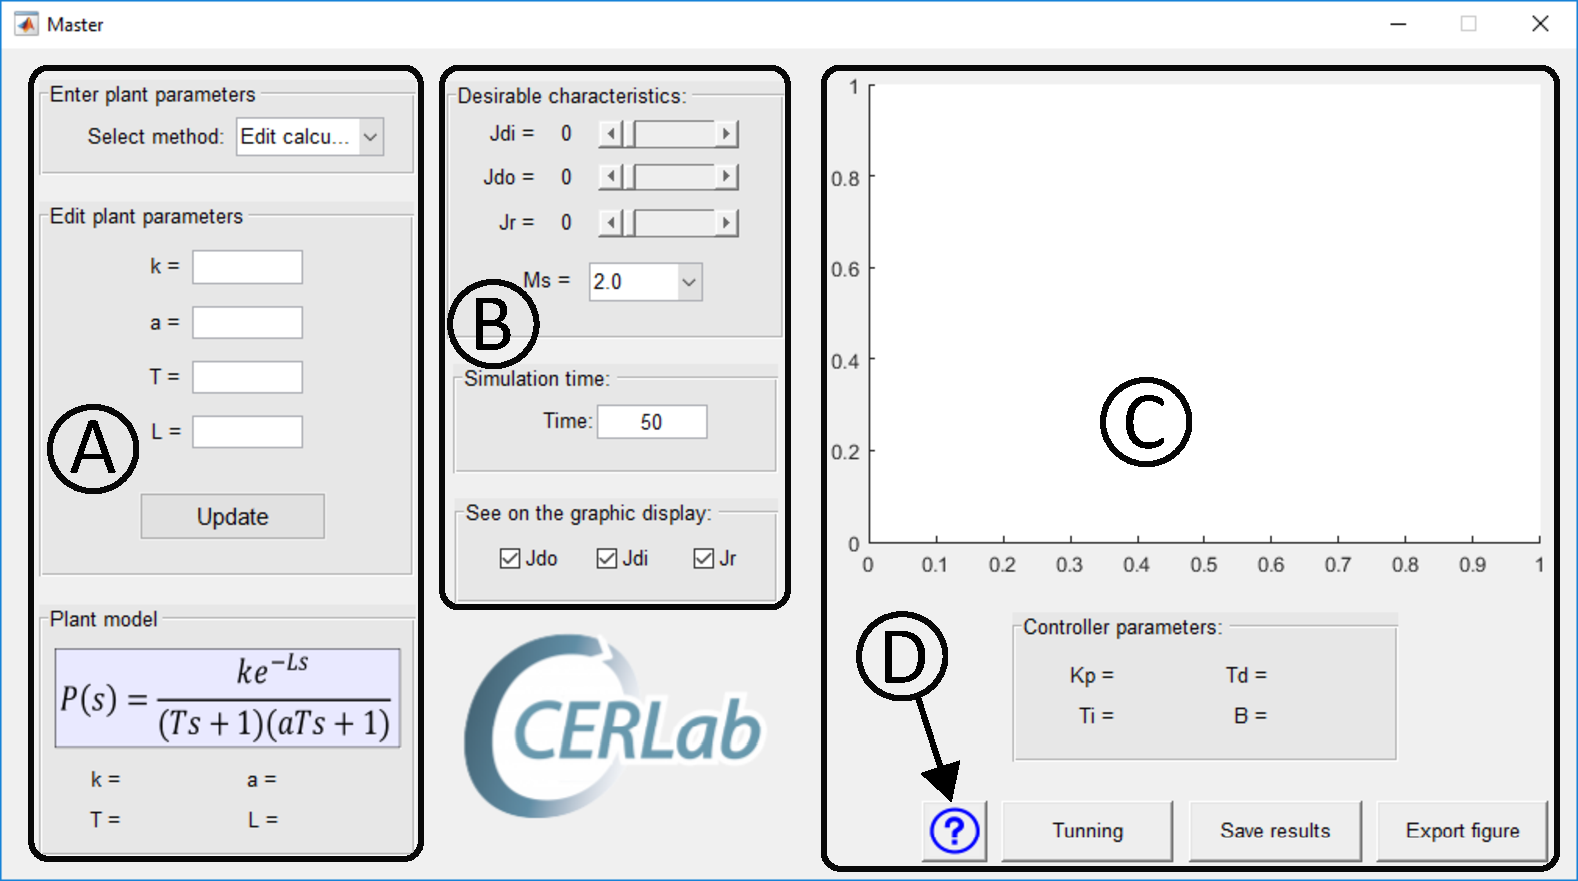
\includegraphics[width=\textwidth]{figuras/gui}
	\caption{The developed \gls{gui} for tuning \gls{pid}.}
	\label{f:gui_tuner}
\end{figure}
%
Fig~\ref{f:gui_tuner}. The \gls{gui} has four main components:
%
\begin{itemize}
	\item ``A'' part was designed to introduce the plant parameters using one of three possible methods: directly introducing its parameters, identifying the model plant from workspace data or identifying a plant model from a comma-separated values (CSV) file. These options are selected in the left top corner of the \gls{gui}.
	\item ``B'' part allows to choose the desirable characteristics for the tuning of a \gls{2dof} \gls{pid}, using the degradation values of $J_{di}$, $J_{do}$ and $J_r$. Also, the closed-loop robustness can be selected by the variable $M_S$.
	\item ``C'' part where the results of ``A'' and ``B'' parts are shown, in graphical and numerical form. It is possible to generate a report of results in plain text format and also to export the generated figure to \matlab.
	\item The ``D'' part is the help manual, that explains the steps for using the \gls{gui}.
\end{itemize}
%

As it can be seen, the user interface is simple and easy to use. Since all the optimization have been performed off-line, the tool is fast in finding the final tuning. The simulation of the closed-loop was computed with a MEX compiled file that solves the delay differential equations\footnote{Compiled MEX files are provided for 64 bits Linux and Windows machines. Other architectures or operating systems should be compiled from source.} using a fourth order Runge-Kutta algorithm.

% \begin{figure}
% \begin{center}
% \includegraphics[width=0.45\textwidth]{figuras/diagrama_proceso}
% \caption{Operating scheme.}
% \end{center}
% \end{figure}
%
\subsection{Plant model}
To model the plant, either from the workspace or from a CSV file, there are two possible ways to find the parameters of the \gls{soptd} method. The first method is using the 123-C algorithm, that uses three points of the reaction curve to find the model~\parencite{Alfaro2006}. The other method uses the optimization toolbox to find the best parameters of the \gls{soptd} transfer function.

The tool was tested by applying an experimental identification of a \gls{soptd} plant described by
\begin{equation}
P(s)=\frac{e^{-0.2s}}{(s+1)(0.5s+1)}.
\label{e:test1}
\end{equation}

The input data correspond to an artificial response produced using \eqref{e:test1}. From the data, the results using the optimization method for system identification presented in %
%
\begin{figure}%[ht]
	\begin{center}
		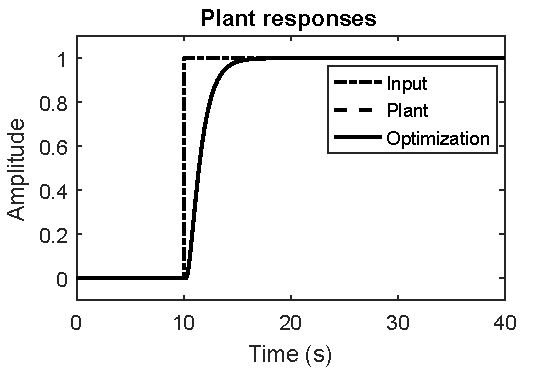
\includegraphics[width=0.65\columnwidth]{figuras/identification}
		\caption{Operating scheme.}
		\label{f:test_res_1}
	\end{center}
\end{figure}
%
%
Fig.~\ref{f:test_res_1}. As it can be seen, the programmed optimization was able to find exactly the model of the plant. It is very important to count with a good model since the interpolation performed in the tool depends heavily from the knowledge of the parameters. The tool is able to find the \gls{pid} controller if the following conditions on the plant are fulfilled:
\begin{equation}
\begin{split}
0.1 &\leq \frac{L}{T} \leq 2 \\
0 &\leq a \leq 1
\end{split}
\label{eq:limits}
\end{equation}
%
\subsection{Example of use.}
\label{sec:example}
%
The \gls{soptd} plant in \eqref{e:test1} is used to verify the correct operation of this tool. A typical closed-loop response is presented in %
\begin{figure}
	\centering
	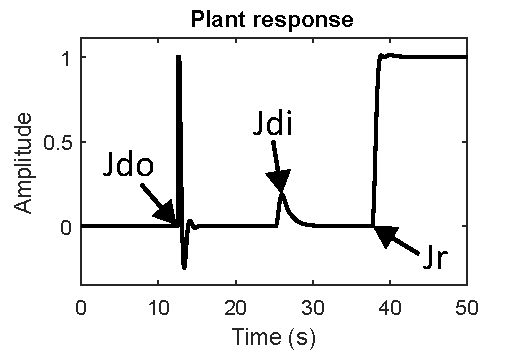
\includegraphics[width=0.65\columnwidth]{figuras/tuning}
	\caption{Control loop response given by the tool.}
	\label{f:control_loop_response}
\end{figure}
Fig~\ref{f:control_loop_response}. As it can be seen, the tool is able to plot the response of each cost function individually.

In order to demonstrate the usefulness of the tool, three different scenarios where tested. On %
%
\begin{table}
	\centering
	\caption{Degradation of parameters.}
	\label{t:jdi_jdo_jr_deg}
	\begin{tabular}{cccccc}
		\toprule
		\multicolumn{1}{c}{\textbf{Parameter}} & \textbf{Figure} & \textbf{Jdi} & \textbf{Jdo} & \textbf{Jr} & \textbf{Ms} \\
		\midrule
		$J_{di}$                      & Fig.~\ref{f:jdi_comp}  & 0.1/0.9      & 0.5          & 0           & 2.0         \\
		$J_{do}$                     &    Fig.~\ref{f:jdo_comp}& 0            & 0.1/0.9      & 0.5         & 2.0         \\
		$J_r$                      &   Fig.~\ref{f:jr_comp} & 0            & 0.5          & 0.1/0.9     & 2.0         \\
		\bottomrule
	\end{tabular}
\end{table}
%
Table~\ref{t:jdi_jdo_jr_deg} the degradation settings are shown. Each case represents the change in the response where one degradation is changed while the others are kept constant. In all cases one of the cost functions degradation is set to zero, this means that, from all the possible optimal tuning that fulfills the degradation requirements, the tool is going to give the tuning that produces the lowest cost function for that particular cost function. When the user selects the desired levels of degradation that do not correspond to the Pareto front (that is, a point so close to the utopia point that does not correspond to the feasible region), a pop-up window appears asking the user to relax the degradation limits.

On %
\begin{figure}
	\begin{center}
		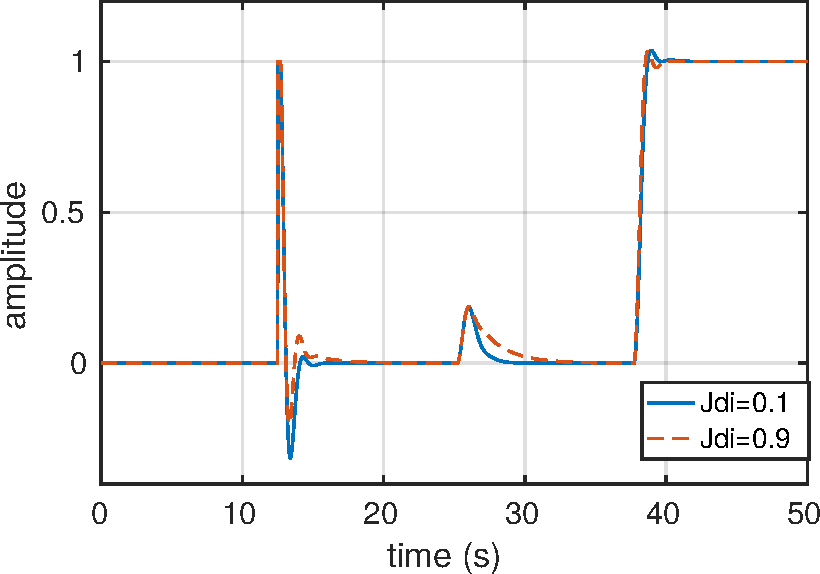
\includegraphics[width=0.65\columnwidth]{figuras/jdi_comp}
		\caption{Variation of $J_{di}$ degradation while keeping the other degradations constant.}
		\label{f:jdi_comp}
	\end{center}
\end{figure}
Fig.~\ref{f:jdi_comp}, two different responses are shown where the allowed degradation of $J_{do}$ is changed while maintaining the other parameter constant. The first response corresponds to a change in $d_o(s)$, the second one is a change in $d_i(s)$ and the final response is a change in $r(s)$. It is clear that, when allowing a higher degradation of $J_{di}$, the response to $d_i(s)$ has a larger \gls{iae}. However, since the responses to each disturbance sources are not independent, varying one degradation settings makes the other responses to vary. However, since the degradation of $J_r$ was kept constant at zero, the tuning given by the tool correspond to the lower value of $J_r$, while satisfying the other degradation levels.

The response of the second case of Table~\ref{t:jdi_jdo_jr_deg} is presented in %
\begin{figure}
	\centering
	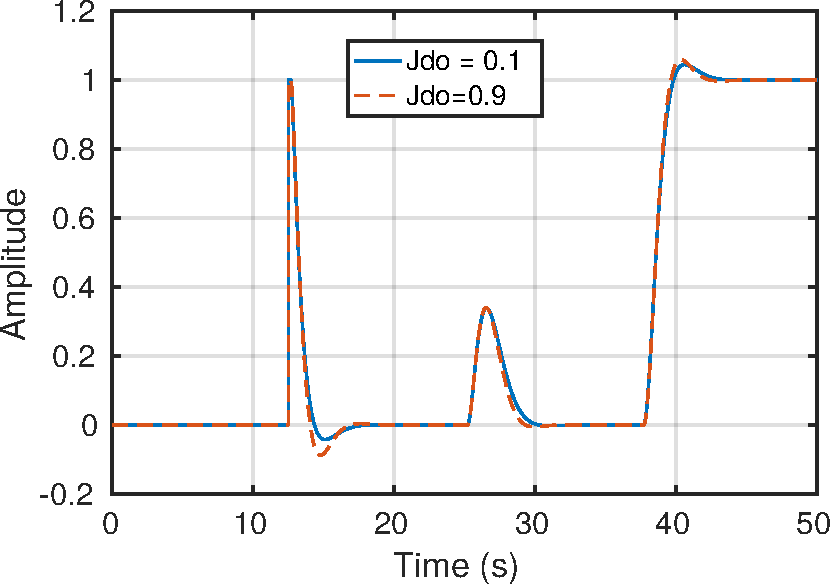
\includegraphics[width=0.65\columnwidth]{figuras/jdo_comp}
	\caption{Jdo comparison.}
	\label{f:jdo_comp}
\end{figure}
%
Fig.~\ref{f:jdo_comp}. This case is interesting because it reflects one of the benefits of analyzing the tuning of \gls{pid} parameters using the Pareto framework. It is clear that, from the point of view of the control engineer, the tuning with a degradation of $J_{do}=0.1$ is more advantageous than for the case of $J_{do}=0.9$, because the degradation on the other responses is minimal while improving the response to a change in $d_o(s)$. Finding this results is easy using the tool presented in this paper, without the need to perform individual optimization for each case.

The third case is presented in %
\begin{figure}
	\centering
	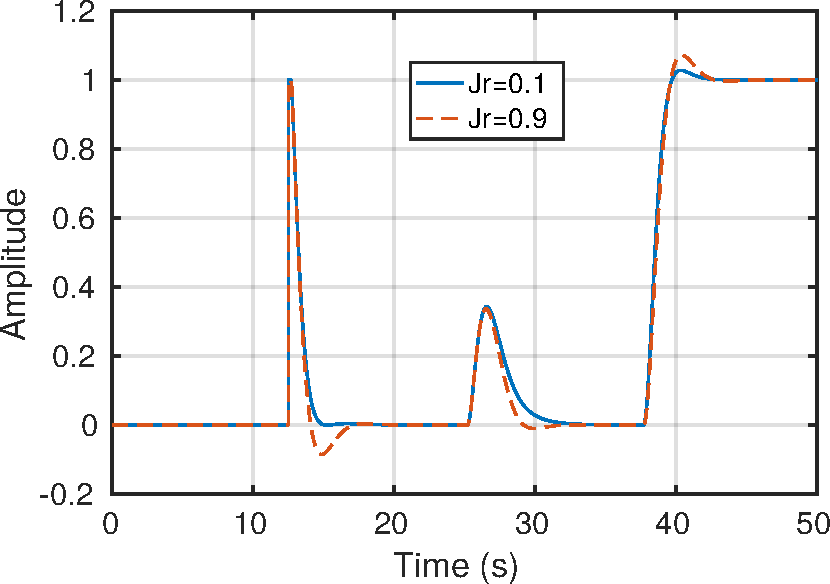
\includegraphics[width=0.65\textwidth]{figuras/jr_comp}
	\caption{Jr comparison.}
	\label{f:jr_comp}
\end{figure}
%
Fig~\ref{f:jr_comp}. In this case is interesting to note that when the allowed degradation of $J_r$ is set to $0.1$, the performance of input disturbance rejection response is also improved. This is important to note because, even thought all three cost function has some kind of antagonism, there are some sections of the Pareto front where is possible to improve two function at the cost of worsening the third function as in this case. The tuning of all the controllers are presented in
%
\begin{table}
	\caption{Obtained parameter of the presented cases.}
	\label{tab:Tunings}
	\centering
	\begin{tabular}{cccccc}
		\toprule
		Case & value & $K_p$ & $T_i$ & $T_d$ & $\beta$\\
		\midrule
		\multirow{2}{*}{$J_{di}$} & $0.1$ & $4.8874$ & $1.1198$ & $0.2566$ & $0.6111$\\
								  & $0.9$ & $4.7449$ & $2.0346$ & $0.2809$ & $0.9095$ \\
		\midrule
		\multirow{2}{*}{$J_{do}$} & $0.1$ & $1.6891$ & $1.2225$ & $0.2738$ & $0.7322$\\
								  & $0.9$ & $1.7400$ & $1.1333$ & $0.2255$ & $0.6647$\\
		\midrule
		\multirow{2}{*}{$J_{r}$}  & $0.1$ & $1.7237$ & $1.4461$ & $0.2522$ & $0.8874$\\
								  & $0.9$ & $1.7166$ & $1.0971$ & $0.2535$ & $0.6685$\\
		\bottomrule
	\end{tabular}
\end{table}
%
Table~\ref{tab:Tunings} for reference. Finally, the last characteristic of the tool is that it is able to save the results of the tuning in plain text. An example of the output report is %
%
\begin{figure}
\centering
\begin{tcolorbox}
%\small
\begin{verbatim}
Characteristic,Value
Plant parameters,Value
K,1
T,1
a,0.5
L,0.2
Desirable characteristics,Value
Jdi,0.26
Jdo,0.24
Jr,0
Ms,2.0
Controller parameters,Value
Kp,4.7206
Ti,1.3629
Td,0.2848
B,0.7379
\end{verbatim}
\end{tcolorbox}
%\normalsize
\caption{Report output.}
\label{f:report_tuning}
\end{figure}
%
presented in Fig.~\ref{f:report_tuning}.